\documentclass[letterpaper,11pt]{article}
\usepackage[utf8x]{inputenc}
\usepackage{enumerate}
\usepackage{enumitem}
\usepackage{fullpage}
\usepackage{amsmath}
\usepackage{hyperref}

\usepackage{pgf}
\usepackage{tikz}
\usetikzlibrary{arrows,shapes,trees}

%opening
\title{Physics 621 (Fall 2017) \\ Homework Assignment 1}
\date{Due: Wednesday September 13, 2017}

\begin{document}

\maketitle

\paragraph*{Mathematics of finite dimensional vector spaces}

All of the following questions are Category C assignment questions; you are welcome to work with others but you should submit your own work.

\begin{enumerate}
  \item Let $A$ be a positive definite Hermitian operator. Show that for all $|\chi\rangle$ and $|\phi\rangle$,
  $$ |\langle \chi|A|\phi \rangle|^2 \le \langle \chi|A|\chi \rangle \langle \phi|A|\phi \rangle. $$
  Under what conditions does the equality hold? (GY 2.9.1)
  \item Let $A(x)$ be an operator that depends on a continuous variable $x$. Define its derivative by
  $$ \frac{dA}{dx} \equiv A'(x) = \lim_{\varepsilon \to 0} \frac{A(x+\varepsilon)-A(x)}{\varepsilon}. $$
  Show that $d(e^{xA})/dx = Ae^{xA}$ if $A' = 0$; if $A$ has an inverse, that
  $$ \frac{d}{dx} A^{-1} = -A^{-1} A' A^{-1}; $$
  and finally, if $A$ and $B$ both depend on $x$, that $d(AB)/dx = A'B + AB'$. (GY 2.9.2)
  \item Let us consider a beam splitter (a mirror which is semi-transpartent to a light wave, a crystal aligned at a Bragg angle for a neutron, etc.) which we assume to be non-absorbing. Waves arrive at the same angle of incidence on the left and right sides of the beam splitter with amplitudes $A_L$ and $A_R$, respectively (the combining beam splitter in the figure). The amplitudes $B_L$ and $B_R$ of the outgoing waves, which are made up of both reflected and transmitted waves, are linearly related to the amplitudes of the incoming waves as
  $$ \left( \begin{array}{c} B_R \\ B_L \end{array} \right) = M' \left( \begin{array}{c} A_R \\ A_L \end{array} \right), \quad M' = \left( \begin{array}{cc} a & b \\ c & d  \end{array} \right). $$
  \begin{enumerate}
    \item Show that $M'$ is unitary and that $\det M' = \exp(i\alpha)$.
    \item Since we are interested in experiments where the outgoing waves interfere, a global phase factor has no physical consequences and $M'$ can be replaced by $M = \exp(-i\theta/2)M'$ with $\det M = -1$. Derive the general form of $M$:
    $$ M = \left( \begin{array}{cc} r & t^* \\ t & -r^* \end{array} \right), |r|^2 + |t|^2 = 1. $$
    \item Show that $M$ can be written as
    $$ M = \left( \begin{array}{cc} |r|e^{i\chi} & |t|e^{-i\phi} \\ |t|e^{i\phi} & -|r|e^{-i\chi} \end{array} \right). $$
    \item Let $\delta_R$ be the difference of the phases of the reflected and transmitted waves for the wave incident from the right only ($A_R = 1$, $A_L = 0$), and let $\delta_L$ be the same phase difference for the wave incident from the left only ($A_R = 0$, $A_L = 1$). Show that
    $$ \delta_R + \delta_L = \pi \pm 2 n \pi, \quad n = 0,1,2,\ldots $$
  \end{enumerate}
 These beam splitters are used in Mach-Zehnder interferometers, devices used to determine the relative phase shift variations between two collimated beams from a single source (see figure). They can be used to visualize flows in wind tunnels.
 \begin{figure}
   \begin{center}
     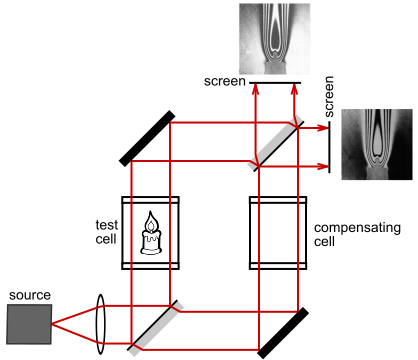
\includegraphics[width=0.5\textwidth]{images/Mach_Zehnder_interferometer}
   \end{center}
   \caption{By Stigmatella aurantiaca - Own work, CC BY-SA 3.0, \url{https://commons.wikimedia.org/w/index.php?curid=25125975}}
 \end{figure}
 \begin{enumerate}[resume]
  \item What is the form of $M$ if the beam splitter is symmetric, $\delta_R = \delta_L = \pi/2$? Show that for suitably chosen phases we can then write the following:
  $$ M = H = \frac{1}{\sqrt{2}} \left( \begin{array}{cc} 1 & 1 \\ 1 & -1 \end{array} \right). $$
\end{enumerate}
  The matrix $H$ is called the \textit{Hadamard matrix or gate} and is widely used in quantum computing. (LB, 2.4.12, with modifications)
  \item In a quantum system with dimension two (for example the two states of a spin-$1/2$ particle) we can assign the value 0 of a quantum bit or \textit{qubit} to the up spin state, and the value 1 to the down spin state:
  $$ |0\rangle \equiv |+1/2\rangle, |1\rangle \equiv |-1/2\rangle. $$
  In contrast to a classical system which can only exist in the state 0 or the state 1, the quantum system can exist in states $|\phi\rangle$ that are linear superpositions of $|0\rangle$ and $|1\rangle$:
  $$ |\phi\rangle = \lambda |0\rangle + \mu |1\rangle, \quad |\lambda|^2 + |\mu|^2 = 1. $$
  A measurement of the $z$ component of the spin will give the result 1 with probability $|\mu|^2$ and the result 0 with probability $|\lambda|^2$. The operations of quantum computers operating on single qubits are unitary transformations of the Hilbert space $\mathcal{H}$ that can be represented as $2 \times 2$ matrices. More generally, when using $n$ qubits we use the Hilbert space $\mathcal{H}^n$ where the unitary operations are represented by $2^n \times 2^n$ matrices.
  \begin{enumerate}
    \item Show that the Hadamard gate maps an input of a single qubit in a basis state (\textit{i.e.} $|0\rangle$ or $|1\rangle$) to a superposition of all possible states with equal probability.
    \item What happens when a single qubit in a basis state (\textit{i.e.} $|0\rangle$ or $|1\rangle$) is sent through two consecutive Hadamard gates? In other words, what is $H^2$? Does this seem weird to you?
    \item What is the matrix representation of the tensor product $H \otimes H$ in the 2-qubit basis $\{|00\rangle ,|01\rangle ,|10\rangle ,|11\rangle\}$ (obtained, for example, by considering two spin-$1/2$ particles)? You may use Mathematica\footnote{This would be a good opportunity to figure out how to install the W\&M campus licensed version at \url{http://www.wm.edu/offices/it/services/software/licensedsoftware/mathstats/wolframmath/index.php}.}
    \item Another fundamental quantum gate is the \textit{controlled NOT} or \textit{cNOT gate}. It operates on the 2-qubit basis $\{|00\rangle ,|01\rangle ,|10\rangle ,|11\rangle\}$ with the following representation:
    $$ \left( \begin{array}{cccc} 1 & 0 & 0 & 0 \\ 0 & 1 & 0 & 0 \\ 0 & 0 & 0 & 1 \\ 0 & 0 & 1 & 0 \end{array} \right). $$
    Explain what this gate does (and where it gets its name).
  \end{enumerate}
\end{enumerate}

\end{document}
